\documentclass{article}
%%%%%%%%%%%%%%%%%%%%%%%%%%%%%%%%%%%%%%%%%%%%%%%%%%%%%%%%%%%%%
% Lecture Specific Information to Fill Out
%%%%%%%%%%%%%%%%%%%%%%%%%%%%%%%%%%%%%%%%%%%%%%%%%%%%%%%%%%%%%
\newcommand{\LectureTitle}{L23: Color}
%\newcommand{\LectureDate}{\today}
\newcommand{\LectureDate}{March 27, 2015}
\newcommand{\LectureClassName}{CS 557}
\newcommand{\LatexerName}{Peter Henderson}
%%%%%%%%%%%%%%%%%%%%%%%%%%%%%%%%%%%%%%%%%%%%%%%%%%%%%%%%%%%%%

% Change "article" to "report" to get rid of page number on title page
\usepackage{amsmath,amsfonts,amsthm,amssymb}
\usepackage{setspace}
\usepackage{Tabbing}
\usepackage{fancyhdr}
\usepackage{lastpage}
\usepackage{extramarks}
\usepackage{chngpage}
\usepackage{soul,color}
\usepackage{mathtools}
\usepackage{graphicx,float,wrapfig}
\usepackage{afterpage}
\usepackage{abstract}
\usepackage{pgfplots}
\usepackage{caption}
\usepackage{listings}
\usepackage{url}

% In case you need to adjust margins:
\topmargin=-0.45in
\evensidemargin=0in
\oddsidemargin=0in
\textwidth=6.5in
\textheight=9.0in
\headsep=0.25in
\tikzstyle{cnstyle}=[domain=0:1, samples=100, ultra thick]

% Setup the header and footer
\pagestyle{fancy}
\lhead{\LatexerName}
\chead{\LectureClassName: \LectureTitle}
\rhead{\LectureDate}
\lfoot{\lastxmark}
\cfoot{}
\rfoot{Page\ \thepage\ of\ \pageref{LastPage}}
\renewcommand\headrulewidth{0.4pt}
\renewcommand\footrulewidth{0.4pt}

%%%%%%%%%%%%%%%%%%%%%%%%%%%%%%%%%%%%%%%%%%%%%%%%%%%%%%%%%%%%%
% Some tools
\newcommand{\enterTopicHeader}[1]{\nobreak\extramarks{#1}{#1 continued on next page\ldots}\nobreak
                                    \nobreak\extramarks{#1 (continued)}{#1 continued on next page\ldots}\nobreak}
\newcommand{\exitTopicHeader}[1]{\nobreak\extramarks{#1 (continued)}{#1 continued on next page\ldots}\nobreak
                                   \nobreak\extramarks{#1}{}\nobreak}

\newlength{\labelLength}
\newcommand{\labelAnswer}[2]
  {\settowidth{\labelLength}{#1}
   \addtolength{\labelLength}{0.25in}
   \changetext{}{-\labelLength}{}{}{}
   \noindent\fbox{\begin{minipage}[c]{\columnwidth}#2\end{minipage}}
   \marginpar{\fbox{#1}}

   % We put the blank space above in order to make sure this
   % \marginpar gets correctly placed.
   \changetext{}{+\labelLength}{}{}{}}

\setcounter{secnumdepth}{0}
\newcommand{\TopicName}{}
\newcounter{TopicCounter}
\newenvironment{Topic}[1][Problem \arabic{TopicCounter}]
  {\stepcounter{TopicCounter}
   \renewcommand{\TopicName}{#1}
   \section{\TopicName}
   \enterTopicHeader{\TopicName}}
  {\exitTopicHeader{\TopicName}}

\setcounter{secnumdepth}{0}
\newcommand{\ExampleSectionName}{}
\newcounter{ExampleSectionCounter}[TopicCounter]
\newenvironment{ExampleSection}[1][Example \arabic{ExampleSectionCounter}]
  {\stepcounter{ExampleSectionCounter}
   \renewcommand{\ExampleSectionName}{#1}
   \section{\ExampleSectionName}
   \enterTopicHeader{\ExampleSectionName}}
  {\exitTopicHeader{\ExampleSectionName}}

\setcounter{secnumdepth}{0}
\newcounter{ExampleBoxCounter}[TopicCounter]
\newcommand{\examplebox}[1]
  {
  % We put this space here to make sure we're disconnected from the previous
   % passage
   \stepcounter{ExampleBoxCounter}
   \noindent\fbox{\begin{minipage}[c]{\columnwidth}#1\end{minipage}}\enterTopicHeader{\ExampleSectionName}\exitTopicHeader{\ExampleSectionName}\marginpar{\fbox{\#\arabic{ExampleBoxCounter}}}
   % We put the blank space above in order to make sure this
   % \marginpar gets correctly placed.
   \vskip10pt
   }

\renewcommand{\contentsname}{{\normalsize Topics Covered}}
\renewcommand{\abstractname}{\LectureTitle\ Summary}
\renewcommand{\absnamepos}{flushleft}

\pgfplotsset{vasymptote/.style={
    before end axis/.append code={
        \draw[densely dashed] ({rel axis cs:0,0} -| {axis cs:#1,0})
        -- ({rel axis cs:0,1} -| {axis cs:#1,0});
    }
}}

%%%%%%%%%%%%%%%%%%%%%%%%%%%%%%%%%%%%%%%%%%%%%%%%%%%%%%%%%%%%%

\begin{document}
\begin{spacing}{1.1}
\newpage

% When topics are long, it may be desirable to put a \newpage or a
% \clearpage before each Topic environment
%\newpage
\begin{Topic}[Color \Roman{TopicCounter}]
RGB values can be rewritten in terms of hue (which colour), saturation (how pure the colour is), and luminance (intensity of colour).
\subsection{Luminance}
The value/intensity of the light. A measure of the average light power over all wavelengths from 400-700 nm. \textit{Note: this says nothing about hue or saturation since it is an average.}
\subsection{Brightness}
\textit{Perceived} luminance (not physically measurable, only measurable behaviourally by asking people how they perceive a colour).

\subsection{What determines a light spectrum?}
The light reflected from a diffusely reflecting surface depends on illumination reflectance.

\subsubsection{OpenGL RGB model}
Doesn't cover the entire spectrum, not based on wavelength.
$$I_{\text{diffuse}}^{RGB}(x) = I_{\text{light}}^{RGB} k_{\text{diffuse}}^{RGB}(x) * \max(\vec{n}, \hat{l})$$
Where $k$ is the diffuse reflectance of the material.
\subsubsection{Physical model considers whole spectrum}
$$E(x, \lambda) = I(x, \lambda) R(x, \lambda)$$
Where $R$ is the reflectance of the material. This is based off the wavelength so covers the full spectrum.

\subsection{How do people/cameras perceive light/colour?}

Two different photoreceptor types: rods and cones.
\subsubsection{Rods}
Used at low light conditions, black/grey/white only.
\subsubsection{Cones}
Used in brighter conditions, perceive colour. Three types of cones based on their light absorbing pigment: L (sensitive to long wavelengths), M (sensitive to medium wavelengths), S (sensitive to short wavelengths).

There is no hard cut-off where one cone starts perceiving light and another stops, instead there is a probability distribution along the wavelength spectrum.

The spectral sensitivity of a camera pixel is built similarly. However, for each pixel there are 4 sensors as per a Bayer pattern (2G, 1R, 1B).

\subsubsection{Principle of Univariance}
A photoreceptor does not know the distribution of wavelengths of photons that it absorbs. Rather it sums the energy of all absorbed photons.

$$I_{RGB}(x,y) = \int C_{RGB}(\lambda) E(x,y,\lambda) d \lambda$$

Where $C_{RGB}(\lambda)$ is the spectral absorption of a photoreceptor and $E(x,y, \lambda)$ is the spectrum of light arriving at cone ($x, y$). Cone absorption $C_{RGB}$ may be easier to understand if we discretize the interval of visible light into N bins. Then the equation becomes:

$$I_{RGB}(x,y) = \sum_\lambda C_{RGB}(\lambda) E(x,y,\lambda)$$

This maps the N-Dimensional spectrum to a 3-D RGB image.

\subsection{Metamers}
It can easily happen that matrix $C$ maps two different radiance spectra $E_1(\lambda)$ and $E_2(\lambda)$ to the same cone absorption triples (i.e. the same RGB point where $CE_1 = CE_2$).  Such spectra $E_1$ and $E_2$ are called \textbf{metamers}. They are visually indistinguishable.

\subsubsection{Colour blindness}
Many people ($\sim 8\%$ of males and $\sim 0.5\%$ of females) are missing a gene for one of the three cone pigments. This leads to three types of colour blindness, depending on which type is missing. Colour blind doesn't mean you can't see colours. Rather, it means that you cannot distinguish some spectra that colour normal people can distinguish. (Such spectra are metamers for the colour blind person.)

\subsection{Colour Displays}
Colour displays (TV, computer, cell phone) have three primary lights (RGB). Their emittance spectra can be represented by an $N \times 3$ matrix $P$ (``phosphor emission spectrum'', or rather basis functions which show what can be displayed on the monitor) such that the net emitted light spectra from a pixel is: $E(\lambda) = P [ I_R, I_G, I_B]^T$ and the captured emission from a camera is: $C P [ I_R, I_G, I_B]^T$ where C is the photoreceptor sensitivity.

Two different displays $P_1$ and $P_2$ will produce different captured RGB values.

\subsection{Anaglyph 3D Displays}
Anaglyph (definition): a stereoscopic photograph with the two images superimposed and printed in different colours, producing a stereo effect when the photograph is viewed through correspondingly coloured filters.

Essentially you want to show two different images to two different eyes so you put an a filter on each eye that filters out one of the two composited images displayed on the screen. This allows you to add depth perception by separating the two images by some distance and perceive a 3D effect.

\subsection{Monochromatic Light}
If you have a monochromatic light (i.e. a laser), then you have the following representation:

$$[I_R, I_C, I_B]^T = C [0, \dots, 1, \dots, 0]^T $$

Where C is the absorption of the cones or the sensitivity of your receptors. Hence, this gives a single colour at that wavelength. Thus, any spectrum $E(\lambda)$ is a linear combination of monochromatic spectra (with positive coefficients).

\[ \left[ \begin{array}{c}
E(\lambda_1)\\
\vdotswithin{\ldots} \\
E(\lambda_n)  \end{array} \right] = E(\lambda_1)
 \left[ \begin{array}{c}
1\\
0\\
\vdotswithin{\ldots} \\
0  \end{array} \right]
+ E(\lambda_2) \left[ \begin{array}{c}
0\\
1\\
\vdotswithin{\ldots} \\
0  \end{array} \right]
+ \dots + E(\lambda_n) \left[ \begin{array}{c}
0\\
0\\
\vdotswithin{\ldots} \\
1  \end{array} \right]
\]

These points map a curve in the $I_{RGB}$ space. If instead of multiplying by a binary vector as in the previous equation, you multiply by a greater scale, you get a ray through that particular point. A chromaticity diagram is a common way of showing this. It's interior is defined by convex combinations of the boundary points. It is another way to show a colour palate.

\begin{center}
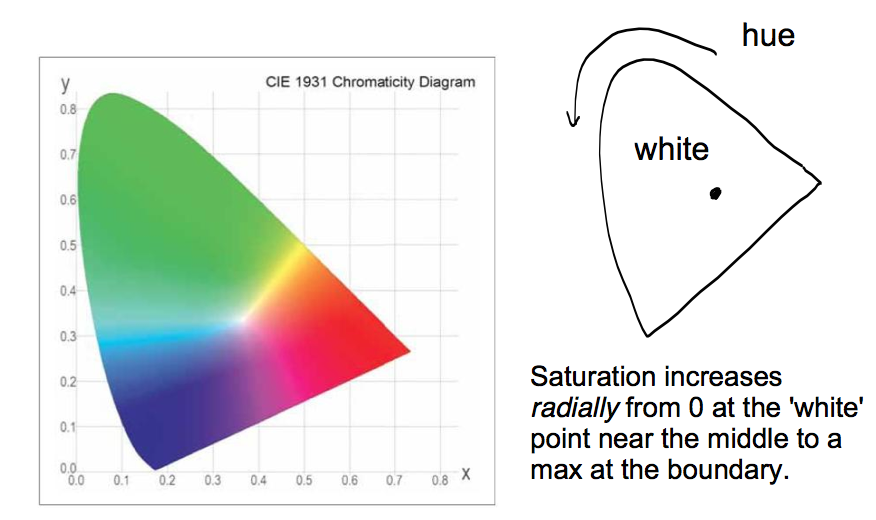
\includegraphics[scale=0.25]{images/chromaticity_diagram}
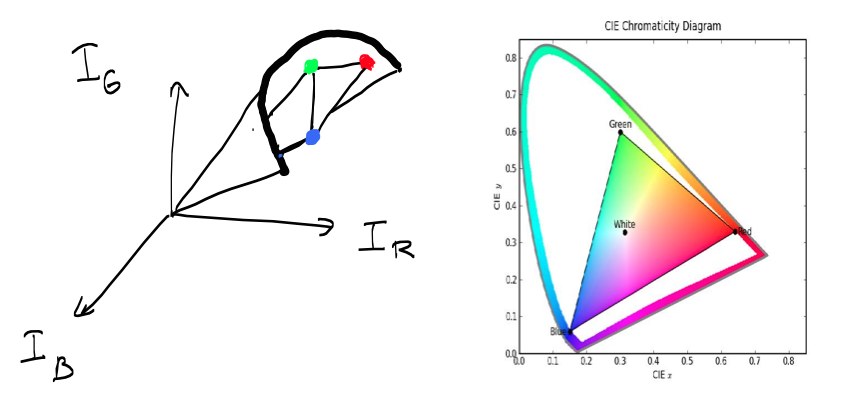
\includegraphics[scale=0.25]{images/display_chromaticity}
\end{center}

A particular display has three spectra that it can produce, namely the columns of matrix $P$ from earlier. The measured RGB values must lie within convex combinations of these three spectra. It must be convex because you cannot have a negative intensity value at a pixel. So you can't reach all the colours seen in the chromaticity diagram above. This essentially cuts out a triangular shape out of the chromaticity diagram.

\textit{Aside: } The chromaticity diagram depends on the matrix $C$, which is different for an eye versus a camera. In 1931, the CIE defined a ``standard observer''. It is related to (but different from) the human cone sensitivities. These cone sensitivities were not known in 1931.

\subsection{Physical versus Perceived Colour}

Perceived intensity doesn't always equal physical intensity. Knowing physical luminance or color of light is useless for survival. The ``color of a material'' (reflectance property) is more important.) We know that physically: surface luminance (x,y) = surface reflectance (x,y) * illumination (x,y)

However, perceptually, the brightness of a surface is often more determined by the perceived reflectance than the perceived luminance. Indeed, when we talk about colour of things we see, we are typically talking about material properties rather than properties of light. Often, when we look at things with the same luminance or intensity, given a darker surrounding it appears brighter even though it's really not.

\end{Topic}

\end{spacing}
\end{document}